%\documentclass{standalone}
\documentclass{article}
\usepackage{tikz}
\usetikzlibrary{calc}
\usetikzlibrary{patterns}

\begin{document}
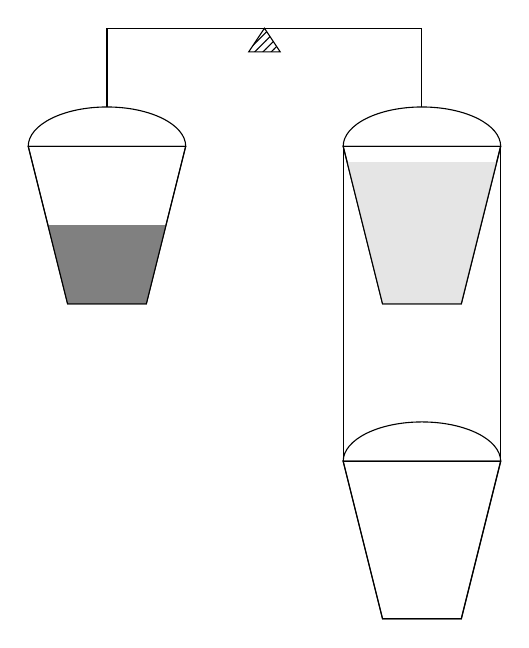
\begin{tikzpicture}

\def\secchio(#1,#2,#3,#4){ % (x, y) dell'apice, percentuale di riempimento e colore
\begin{scope}[shift={(#1,#2)}] %shifta lo zero dii (#1,#2) 
%Traccia l'arco (manico del secchio) %L'origine degli assi e' shiftata prima
\draw (-1,-0.5) arc [start angle=180, end angle=0, x radius=1, y radius=0.5];
%Traccia i contorni del secchio
\draw (-1,-0.5) -- (-0.5,-2.5) -- (0.5,-2.5) -- (1,-0.5) --cycle;
%Colora l'acqua nel secchio di un certo colore
\fill[#4] (-0.5,-2.5) -- (0.5,-2.5) -- ($({0.5*(#3+1))},{2*#3-2.5})$) -- ($({-0.5*(#3+1)},{2*#3-2.5})$); % #4 e' il colore
%Ritraccia i contorni del secchio (altrimenti l'acqua li copre in parte)
%Chiaro che il primo tratto avrei potuto non farlo, ma e' a scopo didattico
\draw (-1,-0.5) -- (-0.5,-2.5) -- (0.5,-2.5) -- (1,-0.5) --cycle;
\end{scope}}

%Disegna i secchi
\secchio(0,0,0.5,gray)
\secchio(4,0,0.9,black!10)
\secchio(4,-4,0,white)

%Disegna le linee
\draw (0,0) -- (0,1) -- (4,1) -- (4,0);
\draw(3,-0.5) -- (3,-4.5);
\draw(5,-0.5) -- (5,-4.5);

%Disegna il perno triangolare
\fill[draw, pattern=north east lines] (2,1) -- (1.8,0.7) -- (2.2,0.7) -- cycle;

\end{tikzpicture}
\end{document}
